% !TEX TS-program = pdflatex
% !TEX encoding = UTF-8 Unicode

% This is a simple template for a LaTeX document using the "article" class.
% See "book", "report", "letter" for other types of document.

\documentclass[11pt]{article} % use larger type; default would be 10pt

\usepackage[utf8]{inputenc} % set input encoding (not needed with XeLaTeX)

%%% Examples of Article customizations
% These packages are optional, depending whether you want the features they provide.
% See the LaTeX Companion or other references for full information.
\usepackage{hyperref}
\usepackage{float}
%%% PAGE DIMENSIONS
\usepackage[margin=1.0in]{geometry} % to change the page dimensions
\geometry{a4paper} % or letterpaper (US) or a5paper or....
% \geometry{margin=2in} % for example, change the margins to 2 inches all round
% \geometry{landscape} % set up the page for landscape
%   read geometry.pdf for detailed page layout information

\usepackage{graphicx} % support the \includegraphics command and options

% \usepackage[parfill]{parskip} % Activate to begin paragraphs with an empty line rather than an indent

%%% PACKAGES
\usepackage{booktabs} % for much better looking tables
\usepackage{array} % for better arrays (eg matrices) in maths
\usepackage{paralist} % very flexible & customisable lists (eg. enumerate/itemize, etc.)
\usepackage{verbatim} % adds environment for commenting out blocks of text & for better verbatim
\usepackage{subfig} % make it possible to include more than one captioned figure/table in a single float
% These packages are all incorporated in the memoir class to one degree or another...
\setlength{\parskip}{0.5em}

%%% HEADERS & FOOTERS
\usepackage{fancyhdr} % This should be set AFTER setting up the page geometry
\pagestyle{fancy} % options: empty , plain , fancy
\renewcommand{\headrulewidth}{0pt} % customise the layout...
\lhead{}\chead{}\rhead{}
\lfoot{}\cfoot{\thepage}\rfoot{}

%%% SECTION TITLE APPEARANCE
\usepackage{sectsty}
\allsectionsfont{\sffamily\mdseries\upshape} % (See the fntguide.pdf for font help)
% (This matches ConTeXt defaults)
%%% ToC (table of contents) APPEARANCE
\usepackage[nottoc,notlof,notlot]{tocbibind} % Put the bibliography in the ToC
\usepackage[titles,subfigure]{tocloft} % Alter the style of the Table of Contents
\renewcommand{\cftsecfont}{\rmfamily\mdseries\upshape}
\renewcommand{\cftsecpagefont}{\rmfamily\mdseries\upshape} % No bold!

%%% END Article customizations

%%% The "real" document content comes below...

\title{Software Engineering Project Weekly Report\\ \textbf{3D-KORN} \\ University of Bourgogne}
\author{Luca Canalini \and Ezequiel De La Rosa \and Benjamin Lalande Chatain \and Roberto Paolella \and Umamaheswaran Raman Kumar \and Savinien Bonheur \and Albert Clerigues Garcia \and Daniel Gonzalez Adell \and Nayee Muddin Khan Dousai \and Pamir Ghimire \and Di Meng
}

\date{November 20, 2016} % Activate to display a given date or no date (if empty),
%         % otherwise the current date is printed 

\begin{document}
\maketitle
\newpage

\section{Tasks Completed}

\begin{itemize}

\item \textbf{Point Cloud Operations Class}
\begin{itemize}
\item \textit{Research and documentation about watertightness}
\item \textit{Conversion from vtk format to stl}
\end{itemize}

\item \textbf{GUI Class}
\begin{itemize}
\item \textit{Research, documentation and test for menubar, toolbar and statusbar.}
\item \textit{Added Kinect stream to the GUI}
\item \textit{Improved the scanning interface}
\end{itemize}

\begin{figure}[h]
\centering
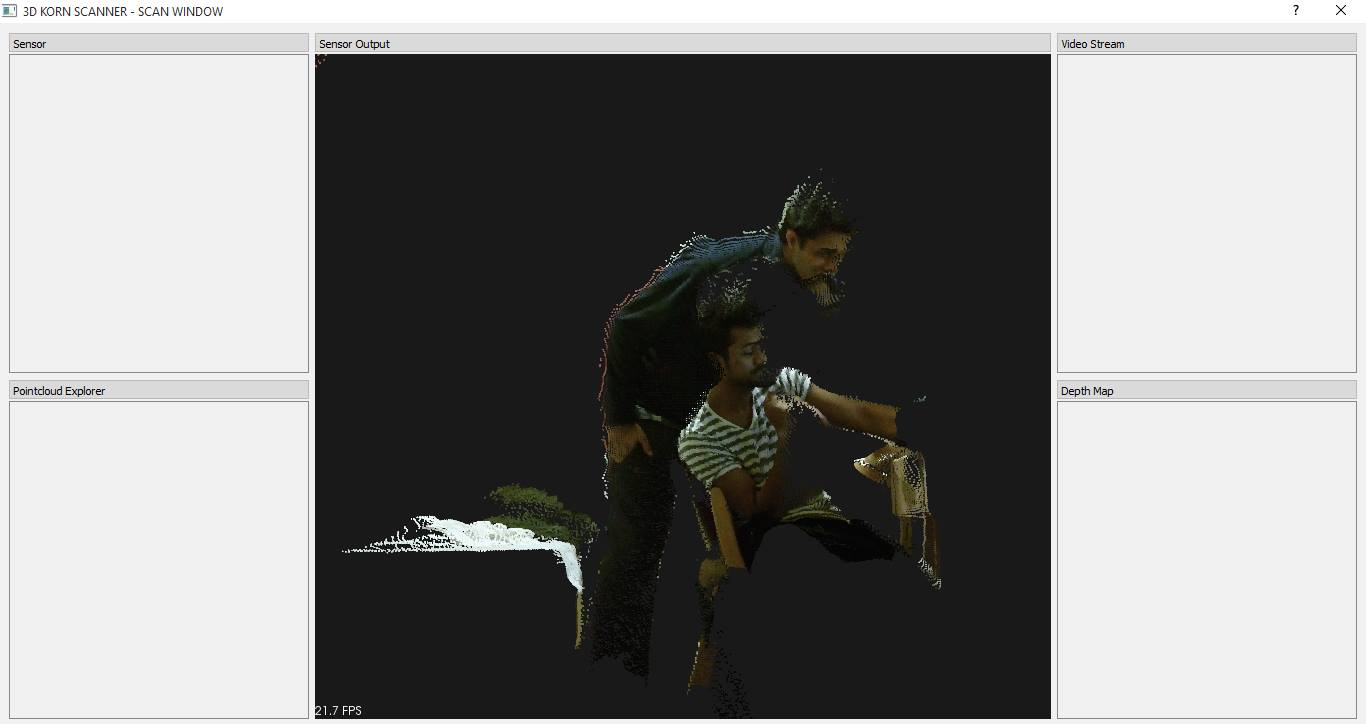
\includegraphics[width=0.7\textwidth]{Scan_Window.png}
\end{figure}

\item \textbf{Scan Registration Class}
\begin{itemize}
\item \textit{Added manual prealignment of scans based on center of turntable rotation and difference of rotation between each scan, which significantly improves the performance of the PCL registration algorithms.}

\begin{figure}[h]
\centering
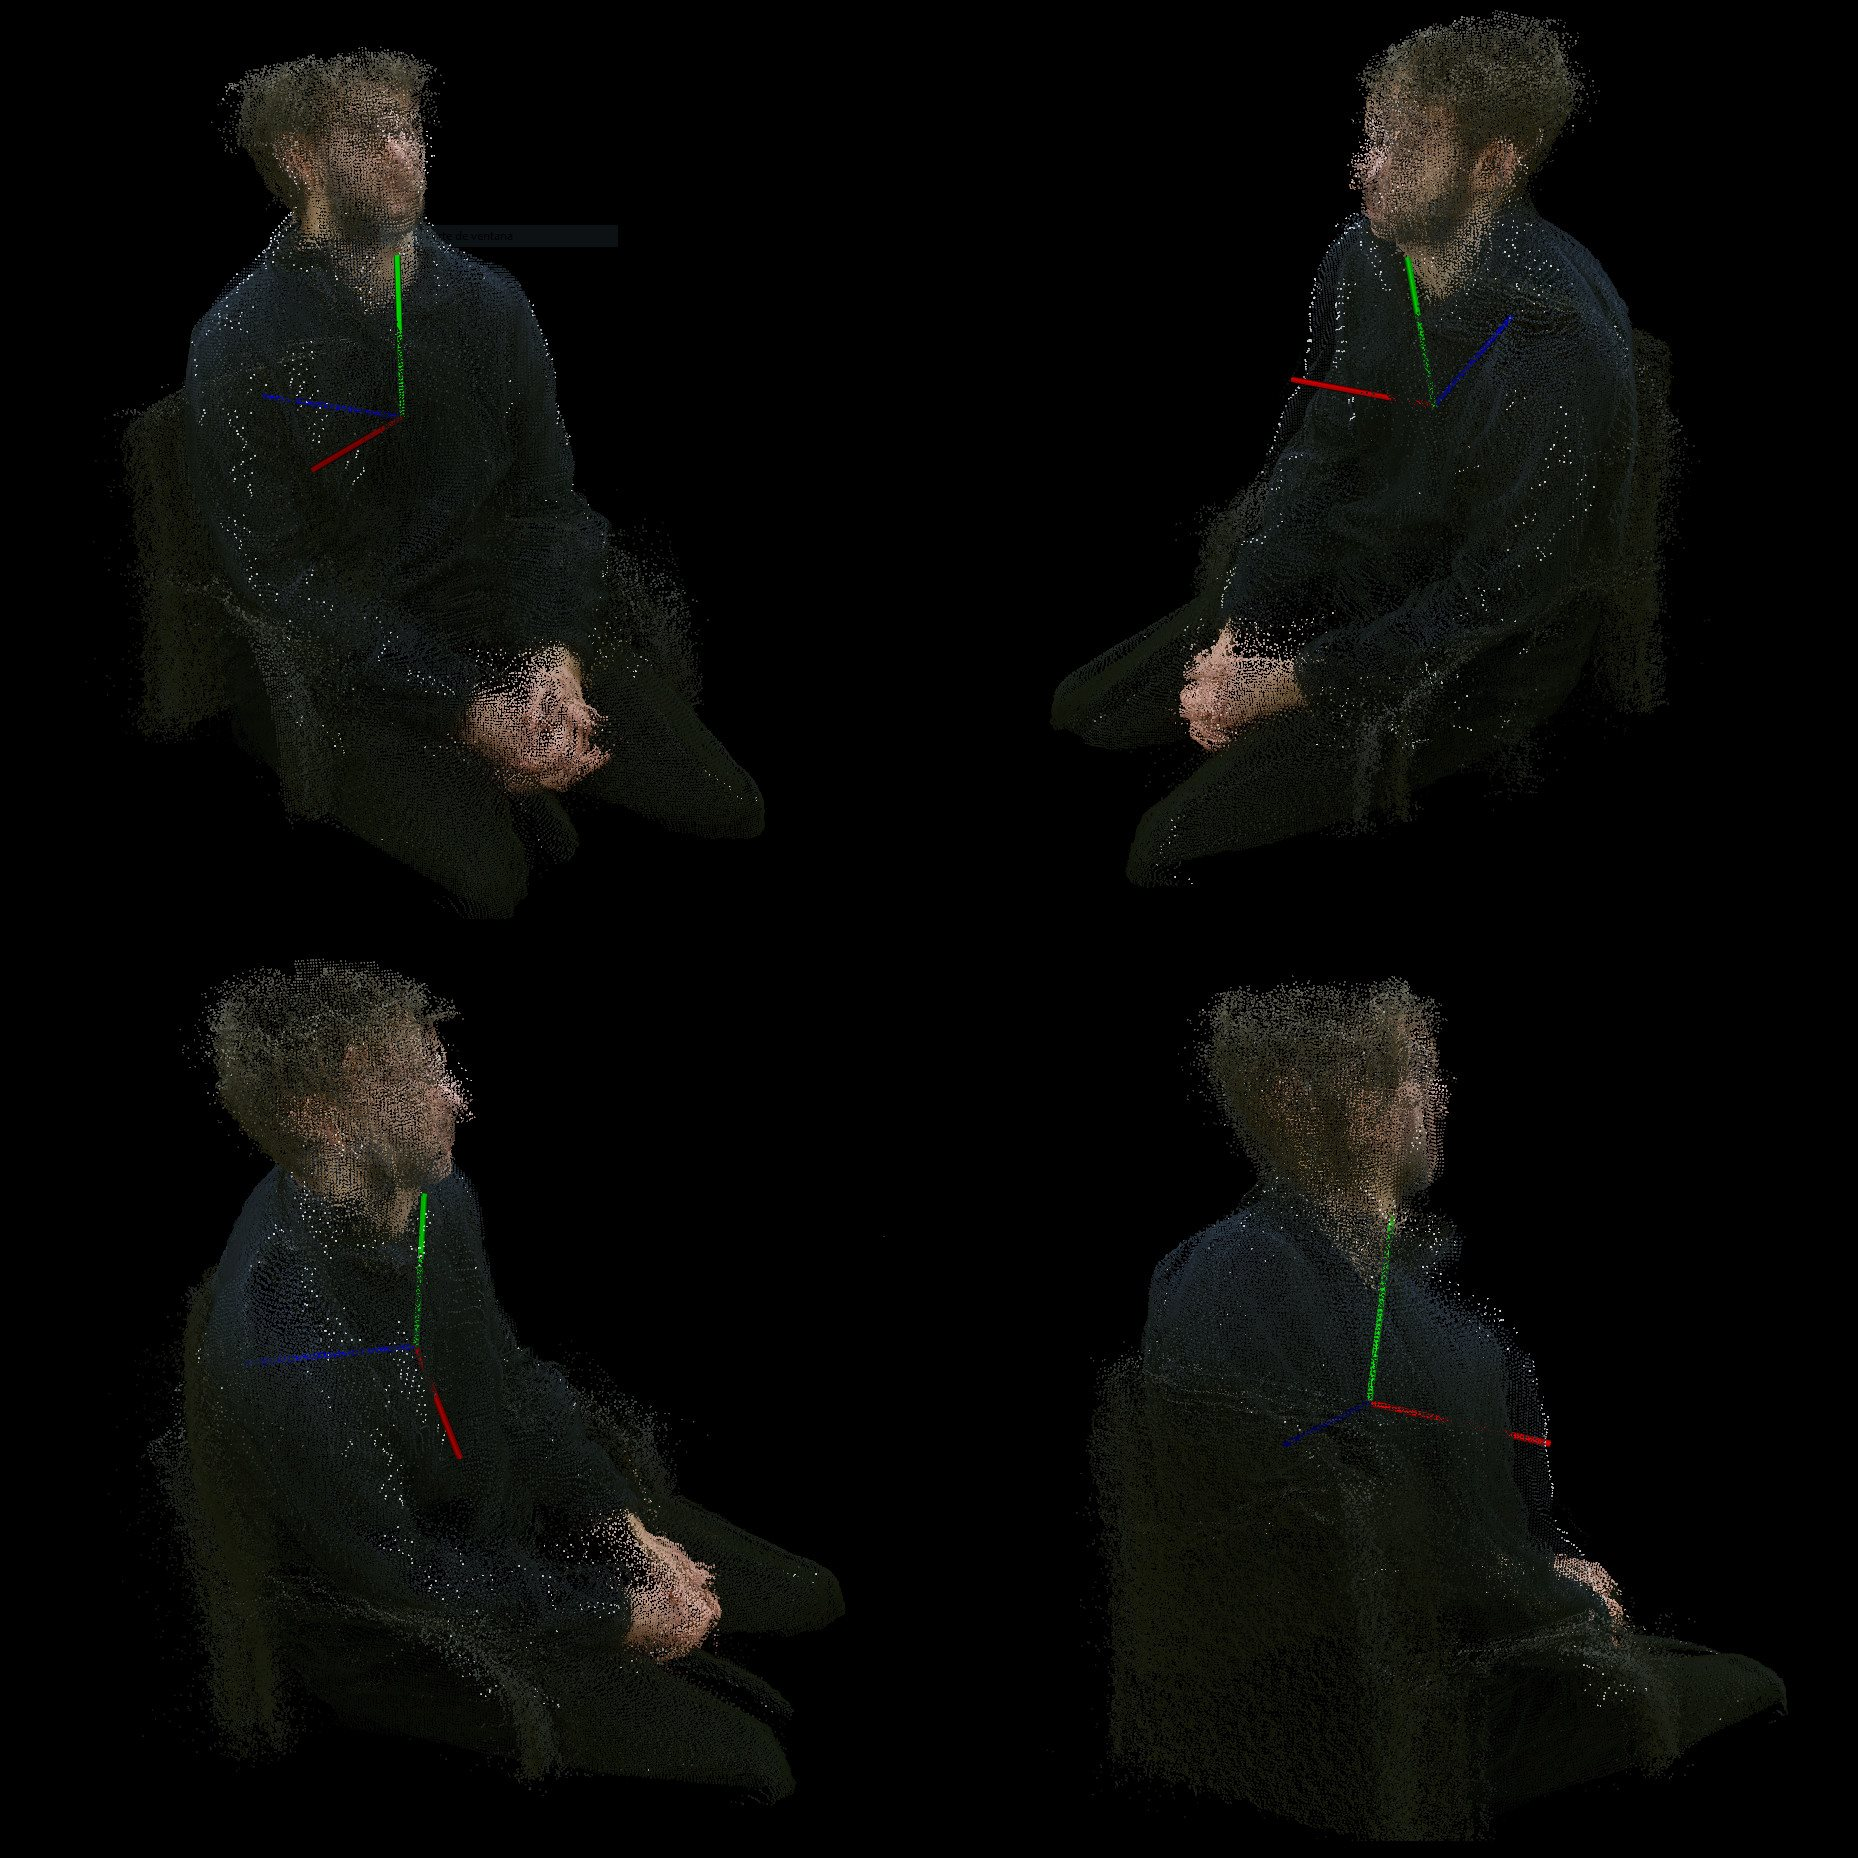
\includegraphics[width=0.45\textwidth]{Scan_Registration.jpg}
\end{figure}

\end{itemize}

\item \textbf{Kinect Controller Class}
\begin{itemize}
\item \textit{Fixed the acquisition of null points}
\item \textit{Defined a cropBox for the acquisition of points}
\item \textit{Completed the TDK\_KinectV2Controller class}
\end{itemize}

\end{itemize}

\section{Main Goals For Next Week}

\begin{itemize}

\item \textbf{Point Cloud Operations Class}
\begin{itemize}
\item \textit{Complete the implementation of watertightness}
\item \textit{Save and Load Class}
\end{itemize}

\item \textbf{GUI Class}
\begin{itemize}
\item \textit{Integration of registration and meshing classes to the GUI}
\item \textit{Improvement of the GUI in term of Friendly User Abilities}
\end{itemize}

\item \textbf{Scan Registration Class}
\begin{itemize}
\item \textit{Research and Documentation for improvements}
\item \textit{Complete the Scan registration}
\end{itemize}

\item \textbf{Kinect Controller Class}
\begin{itemize}
\item \textit{Implement controller functions for R200}
\end{itemize}

\item \textbf{Knowledge transfer session}\\
\\
A knowledge transfer session will be organized this week, where each member will share the acquired knowledge, the implemented features and the work in progress with the rest of the team.

\item \textbf{Platform}\\
\\
A reunion with the different groups for the turntable issue has been organized.\\
The main goal is now to evaluate the feasibility of the proposed design. 4 axes of development have been raised:
\begin{itemize}
\item \textit{The structure of the turntable itself}
\item \textit{The step motor and shield for the Arduino interface}
\item \textit{The traction belt}
\item \textit{The motor encoder}
\end{itemize}


\end{itemize}

\section{Important links}
\begin{itemize}
\item Task allocation and progress  (\url{https://goo.gl/WDHEjf)}
\item Github repository (\url{https://github.com/umaatgithub/3D-KORN})
\end{itemize}
\end{document}
